\documentclass{article}
\usepackage[papersize={8.5in,11in}, margin=0.4in, bottom = 1.3in, headsep=.3in]{geometry}
\usepackage[utf8]{inputenc}
\usepackage{setspace}
\usepackage{amssymb}
\usepackage{amsmath}
\usepackage{physics}
\usepackage{fancyhdr}
\usepackage{ragged2e}
\usepackage[none]{hyphenat}%%%%
\usepackage[scr]{rsfso}
\usepackage{physics}
\usepackage{graphicx}
\usepackage{hyperref}
\usepackage{enumitem}
\usepackage{tikz}
\usetikzlibrary{positioning}

\addtolength{\topmargin}{.5in}

\pagestyle{fancy}
\fancyhf{}
\fancyhead[L]{The Cooper Union \\ESC251 - System Dynamics\\Prof. Luchtenburg}
\fancyhead[R]{Benjamin Aziel  \\Spring 2023\\}
\setlength{\headheight}{23pt}

\newcommand{\Laplace}{\mathscr{L}}
\newcommand{\UnitStep}{\mathscr{U}}
\newcommand{\Integer}{\mathbb{Z}}
\newcommand{\Natural}{\mathbb{N}}
\newcommand{\V}[1]{\overrightarrow{#1}}
\newcommand{\Volume}{{\ooalign{\hfil$V$\hfil\cr\kern0.08em--\hfil\cr}}}

\newcommand{\bicture}[1]{
\begin{center}
    {\includegraphics[height=4cm]{#1}}
\end{center}}
\newcommand{\bitle}[1]{
\bigskip
\large\textbf{#1} \\
\normalsize
}


\begin{document}
\begin{onehalfspacing}

\begin{flushleft}

\bitle{1 - Course Overview}

The course is called Systems Engineering in the course catalog, but Prof. Luchtenburg informally calls it System Dynamics. It's a more apt name for what the course actually covers; if you look up Systems Engineering you'll find a completely different subject.

\medskip

The course text is Ogata's \textit{System Dynamics}, which is a pretty lousy book, I'd recommend reading the first few chapters of Nise or FPE instead. I can provide PDFs if you can't find them yourselves. Read the syllabus, it's pretty in depth.

\medskip

Prof. Luchtenburg \textit{should} put his notes up in the MS Teams Class Notebook and record his lectures. YMMV if you don't bother coming to class.

\bitle{2 - Gradients Make Stuff Flow (Very Hand-Wavey Edition)}

Let's start by throwing out some systems and testing familiarity with first-order systems and simplified models.
\begin{itemize}[noitemsep,topsep=0.5pt]
    \item Emptying a water tank
    \item Cooling of a lightbulb
    \item Discharge of an RC circuit
\end{itemize}

\bicture{1_sys1}

A cylindrical tank is filled to a level \(h\), has a cross-sectional area of \(A\), and an outflow rate of \(Q_\text{out}\). The pressure outside the tank is \(P_{\infty}\). Can we derive a governing equation for this system? Well, we can try with a few physical principles.

\medskip

Let's start with a \textbf{conservation law}. We know there's a volume \(\Volume\) of water proportional to the value of \(h\). Or\dots

\vspace{-0.1in}
\[\Delta \Volume = A \Delta h\]

We'll take the time derivative of that equation to get some more familiar variables. (You might recognize the math here from related rates in Ma111.)

\[\frac{d}{dt} \qty[\Delta \Volume = A \Delta h] = -Q_\text{out}\]

That's not very useful yet. Let's leverage some prior circuits knowledge here...charge moves because of a \textbf{voltage difference} \(\Delta V\), and comparably, fluid moves because of a \textbf{pressure difference}. Ohm's law! We'll come back to that, but the main takeaway here is that the outflow \(Q_\text{out}\) is related to the difference between the pressure inside the tank \(P\) and the atmospheric pressure \(P_\infty\).

\medskip

That circuits analogy comes in handy really often, because it turns out Ohm's law translates directly into fluid flow. 

\[\Delta V = V - V_0 = IR\]
\[\Delta P = P-P_\infty = Q_\text{out} R\]

These are called \textbf{constitutive equations}, or relationships between physical quantities. (The flow is proportional to a level difference, or gradient.)

\medskip

We'll generalize a bit soon, but for now I understand if you don't get it. It's still very hand-wavey.

\medskip

Let's leverage some hydrostatics now. The tank is open to the atmosphere at the top, so we can actually derive an expression for \(P\), the pressure at the base of the tank. We'll also define \(\rho\), the density of the fluid, and \(C\), or capacitance, as \(\frac{A}{\rho g}\), because it ends up being useful in the circuit analogy.\footnote{You'll see this technique leveraged again in ME342.}

\[\Delta P = \rho g \Delta h = \rho g \frac{\Delta \Volume}{A} = \frac{1}{C} \Delta \Volume\]
\[C = \frac{A}{\rho g}\]

OK, I think we're all set. I've been pretty lax with the ``delta's", but it should still be readable. Let me know if things need clarification.

\[\dot{\Volume} = -Q_\text{out}\]
\[C \dot{\Delta P} = - \frac{\Delta P}{R}\]
\[\boxed{RC \dot{\Delta P} + {\Delta P} = 0}\]

This is a really nice differential equation. It looks like the equation for an RC circuit if you've seen those before, with the voltage differentials swapped out for pressure differentials.

\medskip

Let's move onto a second example: the cooling of a lightbulb. When we shut off power to the lightbulb, how can we measure its temperature as it cools to room temperature?

\bicture{1_sys2}

The bulb is initially very hot (with temperature \(T\)) compared to its environment (which has temperature \(T_\infty\)). Heat is flowing outwards at \(\dot{q}_\text{out}\).\footnote{I'm not a fan of the usual notation here, so I'm using \(\dot{q}\) for the flow of heat and \(q\) for heat.} This is seeming very familiar...a temperature difference is driving heat to leave through the resistance \(R\) of the bulb.

\medskip

Let's go through the steps again. What's being conserved here?\footnote{Someone said kinetic energy. What a statistical mechanics-esque answer.} Internal energy! (Or heat, since there's no work in this system.) It might be a bit early in the semester to have seen the capacitive relationship relating heat \(q\) and temperature \(T\) in ESC330, but here it is:

\vspace{-0.1in}
\[\Delta q = C \Delta T\]

Differentiate across the board\dots

\vspace{-0.1in}
\[\frac{d}{dt} \qty(C \Delta T) = C\dot{T} = -\dot{q}_\text{out}\]

And now we're just chugging through the motions. Next is a constitutive relationship (which looks shudderingly close to Ohm's!):

\vspace{-0.1in}
\[\Delta T = T - T_\infty = \dot{q}_\text{out} R\]

Using this and the conservation equation, we construct:

\vspace{-0.1in}
\[\boxed{RC \dot{\Delta T} + \Delta T = 0}\]

Again. Familiar. Very familiar. Maybe there's some unifying theory in the background here.

\bitle{3 - Solving that Damn Equation (and Time Constants)}

We'll generalize that equation to what we call its \textbf{canonical form} \(\tau \dot{y} + y = 0\), a first order differential equation. Let's throw in an initial condition \(y(0)=y_0\) just so we don't have any undetermined constants at the end.

\medskip

To solve this differential equation, we'll guess a solution \(y(t) = ce^{\alpha t}\), find its time derivative \(\dot{y}(t) = \alpha ce^{\alpha t} = \alpha y\), and plug in.

\vspace{-0.1in}
\[\tau \dot{y} + y = 0\]
\[\tau \alpha e^{\alpha t} + e^{\alpha t} = 0\]
\[(\tau \alpha + 1) \; e^{\alpha t} = 0\]
\[\alpha = -\frac{1}{\tau}\]
\[y(t) = ce^{-\frac{t}{\tau}} = y_0 \; e^{-\frac{t}{\tau}}\]

If you look at the graph below, it's just exponential decay from \((0, y_0)\). We call \(\tau\) the \textbf{time constant} of the system, and it's commonly used to describe how quickly an exponential decays or grows. Different systems have different time constants. (Notably, \(RC\) always has units of time). The smaller the time constant, the faster the decay. (Assume for the figure below that \(\tau_1 = 10\) and \(\tau_2 = 5\).)

\bicture{2_exp}

So what happens when we set \(t=\tau\)? Let's plug it in and find out.

\[y(\tau) = y_0 e^{-\frac{\tau}{\tau}} = y_0 e^{-1}\]

So the time constant is the time at which the system response has decayed to \(y_0 e^{-1}\), or approximately 37\% of its initial value. We can also reframe this definition as, ``the time constant is the time at which the system response has lost approximately 63\% of its initial value''. There is a different definition of the time constant for increasing systems that we will explore in the next section.

\bitle{4 - The RC Circuit and Final Generalization}

Say we have an RC circuit with a full capacitor. 

\bicture{2_rc}

The outflow of charge from the capacitor is represented as a negative current:
\vspace{-0.1in}
\[\dot{q} = -I_\text{out}\]

Here's Ohm's law:
\vspace{-0.1in}
\[V = I_\text{out} R = \dot{q} R\]

Finally, we deal in the capacitive relationship (from Ph213):
\vspace{-0.1in}
\[q = C\Delta V\]

Chug everything together and we get:
\vspace{-0.1in}
\[C\dot{\Delta V} = -\frac{\Delta V}{R}\]
\[\boxed{RC \dot{\Delta V} + \Delta V = 0}\]

which is the same equation we've gotten before. (Notably, we don't have to have this equation in terms of the voltage difference; as you'll see in ESC221 this semester, there's a form of the equation in terms of current as well.)

\medskip

Final takeaways:
\begin{itemize}[noitemsep,topsep=0.5pt]
    \item Most first order systems we'll analyze in this class are the same mathematically!
    \item \textbf{Level differences make stuff flow.}
\end{itemize}

\medskip

``Stuff'' isn't the greatest word for something like this, (maybe quantity instead?) but that's the best we have. Stuff can be stored, like charge in a capacitor, or fluid in a tank, or heat in a reservoir. However, by generalizing these quantities, we can create widely applicable rules for modeling first order systems.

\[\text{Stuff} = \text{Capacitance} \times \text{Level Difference}\]
\[\text{Level Difference} = \text{Flow of Stuff} \times \text{Resistance}\]

Also conservation. That's a biggie.
\[\text{Rate of Change of Stuff} = \text{Inflow} - \text{Outflow}\]

We've only discussed scenarios where there isn't anything flowing in thus far. In these cases, to solve nonhomogeneous differential equations, we'll have to use more specialized methods from Ma240 instead of guessing and praying, like the Laplace transform or the method of undetermined coefficients (or as I affectionately call it, MUC).

\bitle{5 - Let's Throw in an Input}

A more simple form of the governing equation for one of these first order systems is:

\vspace{-0.1in}
\[\tau \dot{y} + y = ku\]

when we have a constant input. Think of it as turning on a light switch at time \(t=0\). \(k\) is just a scale factor, and \(u(t)\) is the unit-step function, which is just \(0\) when \(t<0\) and \(1\) when \(t>0\).\footnote{We don't care about what happens at \(t=0\). Stop it.}

\vspace{-0.1in}
\[y(t) = ce^{-\frac{t}{\tau}} + k\]

For the initial condition \(y(0) = y_0\), the undetermined coefficient \(c=y_0 - k\). Here's our updated solution:

\vspace{-0.1in}
\[y(t) = y_0 e^{-\frac{t}{\tau}} + k(1-e^{-\frac{t}{\tau}})\]

When we graph this function for \(y_0 = 0\), we see that it gradually grows towards \(y=k\) as \(t\to\infty\). Now we can analyze exponential growth. You see this behavior everywhere, like when you change a thermostat setting and the temperature slowly creeps towards your choice. This is what we call a \textbf{step response}.

\bicture{2_step}

How could we find the time constant of this response? Let's take a look at what happens to \(y(t)\) at \(t=\tau\).

\vspace{-0.1in}
\[y(\tau) = y_0 e^{-\frac{\tau}{\tau}} + k(1-e^{-\frac{\tau}{\tau}})= y_0 e^{-1} + k(1-e^{-1}) = (y_0-k)e^{-1} + k\]

Anyways, at \(t=\tau\), the system response will have accumulated 63\% of its steady state value.

\medskip

The step input is just one of the test inputs we usually use; we'll look at a few more as the course progresses (such as sinusoidal waves, delta functions, etc.).

\bitle{6 - Our Second Order of Business}

First order systems are honestly pretty boring. When we put in a step input, we just get a pure exponential. We won't be able to get more interesting behavior, like oscillation, because that's just mathematically impossible.\footnote{Prove it!}

\medskip

Second order systems, on the other hand, \textit{can} oscillate by themselves. Try to convince yourself of this mathematically just based on what oscillation is.

\bicture{2_unf}

Mass-spring systems are pretty good models of everything in the world (as long as you use enough mass-spring systems). They're really nice because having a good understanding of ONE mass-spring system provides us with the intuition for more complicated systems. 

\medskip

Say we have a mass-spring system where a mass \(m\) is attached to a wall with a spring \(k\) and a damper \(b\). Gravity isn't ``turned on'', so if you want to visualize the system, that mass is floating. The equation of motion for a positive displacement \(q\) is:\footnote{Prof. Luchtenburg went off on a tangent about Hooke being a genius for realizing that spring motion is linear here. That was pretty funny.}

\vspace{-0.1in}
\[m\ddot{q} = -kq - b\dot{q}\]

Or in its more familiar form:

\vspace{-0.1in}
\[m\ddot{q} + b\dot{q} + kq = 0\]

This is the famed mass-spring equation. Say we have an input - a force \(u\) acting on the mass in the positive direction. Now our equation of motion is:

\vspace{-0.1in}
\[m\ddot{q} + b\dot{q} + kq = u\]

This is a linear differential equation, so we'll solve this by plugging in an educated guess. Let's try \(q(t) = Ae^{st}\).

\vspace{-0.1in}
\[ms^2 Ae^{st} + bs Ae^{st} + kAe^{st} = u\]
\[ms^2 + bs + k = u\]

First, we'll solve the homogeneous equation, or the case where \(u=0\).\footnote{If you're curious why we do this, you can read up on it in a linear algebra textbook. Think it's theorem 3.9 in Friedberg's Linear Algebra.}

\[ms^2 + bs + k = 0\]

This is known as the characteristic (or auxiliary) equation. We can now use algebra to solve for the roots of the equation, and equivalently, the solution of the differential equation.

\[s_{1, 2} = \frac{-b \pm \sqrt{b^2 - 4mk}}{2m}\]

These are also called the \textbf{poles} of the system, but we're getting ahead of ourselves. Let's simplify further.

\[s_{1, 2} = \frac{-b \pm \sqrt{b^2 - 4mk}}{2m} = -\frac{b}{2m} \pm \sqrt{\frac{b^2 - 4mk}{4m^2}} = -\frac{b}{2m} \pm \sqrt\frac{b}{2m}^2 - \frac{k}{m}\]

We define the \textbf{natural frequency} \(\omega_n = \sqrt{\frac{k}{m}}\) and the \textbf{damping ratio} \(\zeta = \frac{b}{2m\omega_n}\). Using these definitions, we can reorganize the mass-spring equation in terms of these variables.

\vspace{-0.1in}
\[m\ddot{q} + b\dot{q} + kq = 0 \qquad \to \qquad \ddot{q} + 2\zeta\omega_n \dot{q} + \omega_n^2 q = 0\]

And the poles of this equation are:

\[s_{1, 2} = -\zeta \omega_n \pm \omega_n \sqrt{\zeta^2 - 1}\]

I just realized this is my second time having this lecture today, so I'm just going to copy-paste my ME301 notes here.

\bitle{6A - Intermezzo - Complex Analysis}

We can locate a complex number in the complex plane using Cartesian coordinates, where \(a\) is the real part and \(b\) is the imaginary part of a point \(z\). The convention is \(z = a+bi = r \cos{\theta}\).

\bicture{2_cpx}

We can interpret this in a polar sense, where \(\theta\) is the angle from the real axis and \(r\) is the distance from the origin to the point. We represent \(z\) as a phasor: \(re^{i\theta}\) using Euler's formula. It's not difficult to translate between Cartesian coordinates and polar coordinates, but I'll dump the formulas here anyway.

\bicture{2_dumb}

\bicture{2_cpx2}

Ah, also the complex conjugate of a number \(z\) is \(\overline{z}\). For \(z = a+bi\), \(\overline{z} = a-bi\).

\bitle{6B - Damping (You Guys are Going to See This Over and Over and Over)}

When \(\zeta = 0\) (or the system is \textbf{undamped}), we have the poles \(s_{1, 2} = \pm i\omega_n^2\). This implies that our solution is a linear combination of sines and cosines, endlessly oscillating, forever and ever. (That's kind of depressing to be honest.)
\medskip

``\textit{What next? Euler guy.}''

\vspace{-0.1in}
\begin{flushright}
    -Prof. Luchtenburg
\end{flushright}

\vspace{-0.1in}
\[x(t) = A_1 e^{i\omega_n t} + A_2 e^{- i \omega_n t} \; \footnote{Apparently \(A_1\) and \(A_2\) are complex conjugates. Don't quote me on that.} = A_1 (\cos(\omega_n t) + i \sin(\omega_n t)) + A_2 (\cos(\omega_n t) - i \sin(\omega_n t))\]
\vspace{-0.3in}
\[= (A_1 + A_2) \cos(\omega_n t) + i(A_1 - A_2) \sin(\omega_n t) = C_1 \cos(\omega_n t) + C_2 \sin(\omega_n t)\]

This reasoning carries over if we pick a damping ratio \(\zeta\) between 0 and 1 (or the system is \textbf{underdamped}). The poles are:

\vspace{-0.1in}
\[s_{1, 2} = -\zeta \omega_n \pm \sqrt{\omega_n^2 (\zeta^2 - 1)} = -\zeta \omega_n \pm i \omega_n \sqrt{1 - \zeta^2} = \sigma \pm i \omega_d\] 

We define the damped frequency \(\omega_d = \omega_n \sqrt{1-\zeta^2}\). (In practice, \(\omega_d \approx \omega_n\), because \(\zeta \ll 1\).) Additionally, we define \(\sigma = i\omega_n\). After substituting these new variables in, our solution becomes:

\vspace{-0.1in}
\[x(t) = A_1 e^{(-\sigma + i\omega_d) t} + A_2 e^{(-\sigma - i\omega_d) t} = e^{-\sigma t} (C_1 \cos(\omega_n t) + C_2 \sin(\omega_n t))\]

In the lattermost form, it's obvious that \(\sigma\) in fact has a use other than bookkeeping; it defines the exponential \textbf{envelope} by which the oscillation decays. An envelope is a function that outlines how a function grows/decays (it's the red line in the figure below).

\bicture{5_env}

Notably, the time constant \(\tau\) of the envelope is equal to \(1/\sigma\). Thus, we can eyeball the value of \(\sigma\) based on how we'd find the time constant (the value \(63\%\) less than the \(y\)-intercept of the envelope).

\vspace{-0.1in}
\[x(t) = e^{-\sigma t} \sin(\omega_d t + \varphi)\]

Most mechanical systems tend to have a very low damping ratio (\(\zeta \simeq O(0.1)\)\footnote{Related rates of growth from Ma111, or big-O notation if you've taken ECE264.}), and as mentioned before, a good rule of thumb is that \(\omega_n = \omega_d\).

\medskip

When we apply some initial conditions (like \(q(0) = q_0\) and \(\dot{q}(0) = v_0\)), our solution becomes:

\vspace{-0.1in}
\[q(t) = e^{\sigma t} \qty(q_0 \cos(\omega_d t) + \frac{\sigma q_0 + v_0}{\omega_d} \sin(\omega_d t))\]

When \(\zeta = 1\), or the system is \textbf{critically damped}, the poles are:

\vspace{-0.1in}
\[s_{1, 2} = -\zeta \omega_n\]

We use a trick from differential equations to fake another linearly independent solution, just chuck on an extra \(t\).

\vspace{-0.1in}
\[q(t) = A_1 e^{-\zeta \omega_n t} + A_2 t e^{-\zeta \omega_n t}\]

This doesn't really happen in the real world, but it's nice to cover all our bases. How about when \(\zeta > 1\)? We call this case \textbf{overdamped}, because our poles are:

\vspace{-0.1in}
\[s_{1, 2} = -\zeta \omega_n \pm \omega_n \sqrt{\zeta^2 - 1}\]

Both poles are negative here! Our solution is:

\vspace{-0.1in}
\[q(t) = A_1 e^{s_1 t} + A_2 e^{s_2 t}\]

\bitle{7 - Pole Plots}

I've been emphasizing poles a lot in the last few pages, but why? What's the importance of these seemingly arbitrary values? In fact, we can infer the dynamics of a system based on its poles.\footnote{This is the crux of a lot we do in ME351. If any of you remember what an eigenvalue is from Ma110, that'll come in handy in a bit.}

\medskip

To analyze poles, we use a graphical tool called a \textbf{pole plot}, the plot of the roots of the characteristic equation on the complex plane. Let's go down the list:

\begin{itemize}[noitemsep]
    \item When both poles are on the imaginary axis, the system is undamped.
    \item When both poles are off the real axis, the system oscillates. If they're to the left of the imaginary axis, it'll decay exponentially (underdamped), and if they're to the right of the imaginary axis, it'll grow exponentially.
    \item If both poles are on the real axis to the left of the imaginary axis, it's overdamped.
    \item Rule of thumb: if there is ANY pole to the right of the imaginary axis, the response blows up.
\end{itemize}

Here's a nice chart from FPE. Complex conjugates are omitted for simplicity.

\begin{center}
    {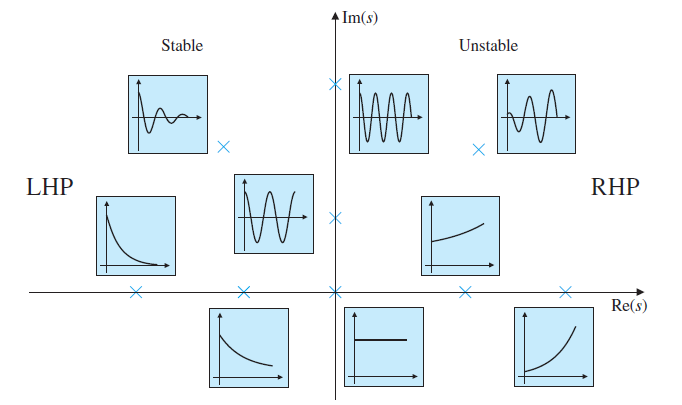
\includegraphics[height=8cm]{7_fpe}}
\end{center}

\bitle{8 - Discriminants}

I'm going to stray off from Prof. Luchtenburg for a second because \textit{I} think this is useful. Your opinion might differ, if so, skip it.

\textbf{WIP}

\end{flushleft}
\end{onehalfspacing}
\end{document}
